\chapter{The Jac Programming Language}

To articulate the sourcer spells made possible by the wand that is Jaseci, I bestow upon thee, the Jac programming language. (Like the Harry Potter~\cite{harrypotter} simile there? Cool, I know ;-) )
\par
The name Jac take was chosen for a few reasons.
\begin{itemize}
    \item ``Jac'' is three characters long, so its well suited for the file name extention \texttt{.jac} for Jac programs.
    \item It pulls its letters from the phrase \textbf{JA}seci \textbf{C}ode.
    \item And it sounds oh so sweet to say ``Did you \gls{grok} that \gls{sick} Jac code yet!'' Rolls right off the tongue.
\end{itemize}
\par
This chapter provides the full deep dive into the language. By the end, you will be fully empowerd with Jaseci wizardry and get a view into the key insights and novelty in the coding style.

%%%%%%%%%%%%%%%%%%%%%%%%%%%%%%
\section{Getting the Basics Out of the Way}
First lets quickly dispense with the mundane. This section covers the standard table stakes fodder present in pretty much all languages. This stuff must be included for completeness, however you should be able to speed read this section.  If you are unable to speed read this, perhaps you should give visual basic a try.

%%%%
\subsection{The Obligatory Hello World}
\printfigHelloWorldBaby
Let's begin with what has become the unofficial official starting point for any introduction to a new language, the ``hello world'' program. Thank you Canada for providing one of the most impactful contributions in computer science with ``hello world'' becaming a meme both technically and socially. We have such love for this contribution we even tag or newborns with the phrase as per Fig.~\ref{fig:hello_baby}. I digress. Lets now \gls{christen} our baby, Jaseci, with its ``Hello World'' expression.

\jaccode{hello_world.jac}{Jaseci says Hello!}

Simple enough right? Well let's walk through it. What we have here is a valid Jac program with a single walker defined. Remember a walker is our little robot friend that walks the nodes and edges of a graph and does stuff. In the currly braces, we articulate what our walker should do. Here we instruct our walker to utilize the standard library to call a print function denoted as \texttt{std.out} to print a single string, our star and esteemed string, ``Hello World.'' The output to the screen (or wherever the OS is routing it's standard stream output) is simply,

\shellout{hello_world.jac.output}

And there we have the most useless program in the world. Though\dots technically this program is AI. Its not as intelligent as the machine depicted in Figure~\ref{fig:hello_baby}, but one that we can understand much better (unless you speak ``\gls{goo goo gaa gaa}'' of course). Let's move on.

%%%%
\subsection{Basic Arithmetic Operations}
Next we should cover the he simplest math operations in Jac. We build upon what we've learned so far with our conversational AI above.

\jaccode{jac_arith.jac}{Basic arithmetic operations}

The output of this groundbreaking program is,

\shellout{jac_arith.jac.output}

Jac Code~\ref{jac:jac_arith.jac} is comprised of basic math operations. The semantics of these experisions are pretty much the same as anything you may have seen before, and pretty much match the semantics we have in the Python language. In this Example, we also observe that Jac is an untyped langauge and variables can be delcared via a direct assignment; also very Python'y. The comma separated list of the defined variables \texttt{a} - \texttt{e} in the call to \texttt{std.out} illustrate multiple values being printed to screen from a single call.
\par
Additionally, Jac supports power and modulo operations.

\jaccode{jac_more_arith.jac}{Additional arithmetic operations}

Jac Code~\ref{jac:jac_more_arith.jac} outputs,

\shellout{jac_more_arith.jac.output}

Here, we can also observe that, unlike Python, whitespace does not mater whatsoever. Languages utilizing whitespace to express static scoping should be criminalized. Yeah, I said it, see Rant~\ref{rant:whitespacesucks}. Anyway, A corollary to this design decision is that every statement must end with a ``\texttt{;}''. The wonderful \texttt{;}, A nod of respect goes to \texttt{C/C++/JavaScript} for bringing this beautiful code punctuation to the masses. Of course the \texttt{;} as code punctuation was first introduced with \texttt{ALGOL 58}, but who the heck knows that language. It sounds like some kind of plant species. \Gls{bleh}. Onwards.

\begin{nerd}
    Grammar~\ref{gram:jac.g4:126:132} shows  the lines from the formal grammar for Jac that corresponds to the parsing of arithmetic.
    \gramcoderange{jac.g4}{Jac grammar clip relevant to arithmetic}{126}{132}
\end{nerd}

%%%%
\subsection{Comparison, Logical, and Membership Operations}
Next we review the comparison and logical operations supported in Jac. This is relatively straight forward if you've programmed before. Let's summarize quickly for completeness.
\jaccode{jac_compare.jac}{Comparision operations}
\shellout{jac_compare.jac.output}
In order of appearnce, we have tests for equality, non equality, less than, greater than, less than or equal, and greater than or equal. These tools prove indispensible when expressing functionality through conditionals and loops. Additionally,

\jaccode{jac_logical.jac}{Logical operations}
\shellout{jac_logical.jac.output}
Jac Code~\ref{jac:jac_logical.jac} presents the logical operations supported by Jac. In oder of appearnce we have, boolean complement, logical and, logical or, another way to express and and or (thank you Python) and some combinations. These are also indispensible when using conditionals.

[NEED EXAMPLE FOR MEMBERSHIP OPERATIONS]

\begin{nerd}
    Grammar~\ref{gram:jac.g4:116:124} shows the lines from the formal grammar for Jac that corresponds to the parsing of comparison, logical, and membership operations.
    \gramcoderange{jac.g4}{Jac grammar clip relevant to comparison, logic, and membership}{116}{124}
\end{nerd}

%%%%
\subsection{Assignment Operations}
Next, lets take a look at assingment in Jac. In contrast to equality tests of \texttt{==}, assignment operations copy the value of the right hand side of the assignment to the variable or object on the left hand side.
\jaccode{jac_assign.jac}{Assignment operations}
\shellout{jac_assign.jac.output}
As shown in Jac Code~\ref{jac:jac_assign.jac}, there are a number of ways we can articulate an assinment. Of course we can simply set a variable equal to a particular value, however, we can go beyond that to set that assinment relative to its original value. In particular, we can use the short hand \texttt{a += 4 + 4;} to represent \texttt{a = a + 4 + 4;}. We will describe later an additional assignment type we call the copy assign. If you're simply dying of curiousity, I'll throw you a bone. This \texttt{:=} assignment only applies to nodes and edges and has the semantic of copying the member values of a node or edge as opposed to the particular node or edge a variable is pointing to. In a nutshell this assignment uses pass by value semantics vs pass by reference semantics which is default for nodes and edges.

\begin{nerd}
    Grammar~\ref{gram:jac.g4:104:112} shows the lines from the formal grammar for Jac that corresponds to the parsing of assignment operations.
    \gramcoderange{jac.g4}{Jac grammar clip relevant to assignment}{104}{112}
\end{nerd}



%%%%
\subsection{Precedence in Jac}
\printtabPrecedence
At this point in our discussion its important to note the precedence of opperations in Jac. Table~\ref{tab:jacprecedence} summarizes this precedence. There are a number of new and perhaps interesting things that appear in this table that you may not have seen before. [JOKE] For now, don't hurt yourself trying to understand what they are and mean, we'll get there.



%%%%
\subsection{Foreshadowing Unique Graph Operations}
\jaccode{jac_preview.jac}{Preview of graph operators}
\begin{figure}
    \centering
    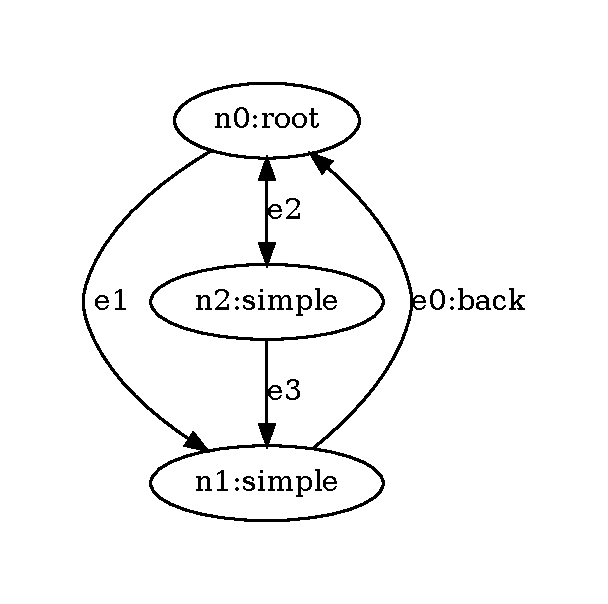
\includegraphics[width=.5\linewidth]{assets/dot/jac_preview.dot.pdf}
    \caption[]{A preview of whats to come in Jac Land!}
    \label{dot:jac_preview}
\end{figure}